\documentclass[a4paper]{article}
\usepackage[utf8]{inputenc}
\usepackage[russian,english]{babel}
\usepackage[T2A]{fontenc}
\usepackage[left=10mm, top=20mm, right=18mm, bottom=15mm, footskip=10mm]{geometry}
\usepackage{indentfirst}
\usepackage{amsmath,amssymb}
\usepackage[italicdiff]{physics}
\usepackage{graphicx}
\graphicspath{{images/}}
\DeclareGraphicsExtensions{.pdf,.png,.jpg}
\usepackage{wrapfig}
\usepackage{float}
\usepackage{subcaption}
\usepackage{enumitem}
\usepackage{pdflscape}
\usepackage{caption}
\usepackage{array}
\captionsetup[figure]{name=Рисунок}
\captionsetup[table]{name=Таблица}

\title{\underline{Отчет о выполненой лабораторной работе 2.2 (2.3)}}
\author{Воронин Денис, Б04-407}

\begin{document}

\maketitle

\textbf{Цель работы:} измерить спектры поглощения паров йода, выделить серии электронно-колебательных переходов, определить параметры потенциала межъядерного взаимодействия в двухатомной молекуле йода.

\textbf{В работе используются:} оптическая скамья, линза, монохроматор УМ-2 оборудованный системой цифровой регистрации изображения спектра (зеркальный цифровой фотоаппарат присоединённый к компьютеру), программное обеспечение для работы с данными raw-файлов, газоразрядные ртутная и неоновая лампы, лампа накаливания и герметичные кюветы с парами йода.


\section{Аннотация}

По окончании работы должны будем прокалибровать барабан спектрометра по спектрам неона и ртути. Определить координаты линый бальмеровской серии атомарного водорода и по результатам измерений рассчитать постоянную Ридберга. Определить координаты нескольких линий молекулярного спектра йода и по результатам измерений вычислить энергию колебательного кванта молукулы йода и энергию ее ддиссоциации в 
основном и возбужденном состояниях.

\section{Теоретические сведения}

Атом водорода - простейшая атомная система. Для него уравнение Шредингера может быть решено точно. 
Квантово - механическая задача об относительности движения электрона сводится к задаче о движении частицы с относительной массой \[
\mu = m_e M / (m_e + M)
\]

в кулоновском поле. Длины волн спектральных линий водородного атома описывается формулой:
\[
\frac{1}{\lambda_{mn}} = R Z^2 \left( \frac{1}{n^2} - \frac{1}{m^2} \right) \tag{1}
\]

Формула (1) называется обобщенной формулой Бальмера.\par

Для объяснения спектра атома водорода Нильс Бор предположил $\textbf{теорию атома}$ в основу которой положил 3 постулата:

\begin{itemize}
	\item Сущ стационарные орбиты, при движениии по которым электром  не излучает энергии
	\item В втоме осущ только те орбиты, для которых момент движения \[
L = n\hbar;
\]
	\item Излучение и поглощение происходит при переходе из одного стац сост в другое, а тчатоста  излуч (поглощения) энергии связана с разностью энергий в стац сост как:
\[
h\nu = E_2 - E_1,
\]
\end{itemize}


В работе изучается серия Бальмера. Энергетические состояния водородоподобного атома определяются формулой:

\[
E_n = -\frac{2\pi^2 m_e e^4 Z^2}{h^2} \frac{1}{n^2} \tag{2}
\]
 
\newpage

\begin{figure}[!hb]
	\centering
	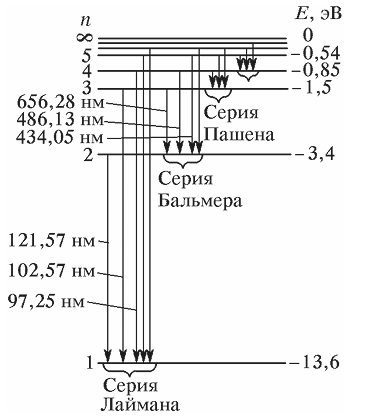
\includegraphics[width=0.3\linewidth]{p4.png}
	\caption{Уровни энергии атома водорода и образование спектральных серий}
	\label{pic_2}
\end{figure}

Знание энергетических состояний атома позволяет по формуле (2) определить возможные частоты его излучения и объяснить наблюдаемые спектральные закономерности (рис.1).\par

По полной энергии и нахождения ее экстремума найдем Боровский радиус:

\[
r_{\text{Б}} = \frac{\hbar^2}{Z m_e e^2} \tag{3}
\]

Зная (3) и подставив ее в выражение полной энергии найдем энергию основного состояния:

\[
E = -\frac{m_e e^4}{2\hbar^2} Z^2 = -R Z^2 \tag{4}
\]

Аналогично можно найти энергию возбужденных состояний:

\[
r_n = \frac{n^2 \hbar^2}{Z m_e e^2} \tag{5}
\]

\[
E_n = -\frac{m_e Z^2 e^4}{2\hbar^2} \frac{1}{n^2} = -R \frac{Z^2}{n^2} \tag{6}
\]

Положение линий спектра водорода и дейтерия различаются. Это называется изотропический сдвиг. Это происходит из-за того, что электрон движется не вокруг ядра, а вокруг ЦМ системы. Величина сдвига межде вородом и дейтерием определяется по формуле:

\[
\frac{\Delta\lambda}{\lambda} = \frac{m_e}{m_p} \frac{A_{\mathrm{D}} - A_{\mathrm{H}}}{A_{\mathrm{D}} A_{\mathrm{H}}} \simeq \frac{m_e}{2M_{\mathrm{H}}} \tag{7}
\]

$\textbf{Йод}$\par

Молукулы обладают более богатым спектром возбужденныз состояний, чем изолированные атомы, так как в молекулах могут возбуждаться дополнительные степени свободы. В перовом приближении энергии молукул представляюися в виде:

\[
E = E_{\text{эл}} + E_{\text{колеб}} + E_{\text{вращ}} \tag{8}
\]

Волновая функция молекулы может быть представлена в виед произведения 3-х волновых функций:

\[
\psi = \psi_{\text{эл}} \cdot \psi_{\text{колеб}} \cdot \psi_{\text{вращ}} \tag{9}
\]

Можно рассмотреть как соотносятся между собой величины электронной, колебательной и вращательной энергии молекулы:

\[
\frac{\omega_{\text{колеб}}}{\omega_{\text{эл}}} \approx \sqrt{\frac{m}{M}} \tag{10}
\]


\[
\frac{\omega_{\text{вращ}}}{\omega_{\text{эл}}} \approx \frac{m}{M} \tag{11}
\]

Объединяя оценки получим:

\[
\omega_{\text{эл}} : \omega_{\text{колеб}} : \omega_{\text{вращ}} \approx 1 : \sqrt{\frac{m}{M}} : \frac{m}{M} \approx 1 : 10^{-3} : 10^{-6}.
\]

\newpage

\section{Экспериментальная установка}

Для наблюдения спектра водорода используется установка, изображённая на Рис. 2 А. Источником света для наблюдения служит водородная трубка Н-образной формы, в состав газа которой добавлены водные пары для увеличения яркости интересующих нас линий. Источник Л помещается на оптическую скамью вместе с конденсером К, так что свет концентрируется на входной щели 1. Далее через коллиматорный объектив 2 свет попадает на сложную спектральную призму, состояющую из призм П$_1$, П$_2$ и П$_3$. Первые две призмы обладают большой дисперсией, а промежуточная П$_3$ поворачивает лучи -- такое устройство позволяет складывать дисперии П$_1$ и П$_2$. После прохождения призмы свет попадает в зрительную трубу 4-5, объектив которой даёт изображение входной щели различных цветов.

\begin{figure}[!hb]
	\centering
	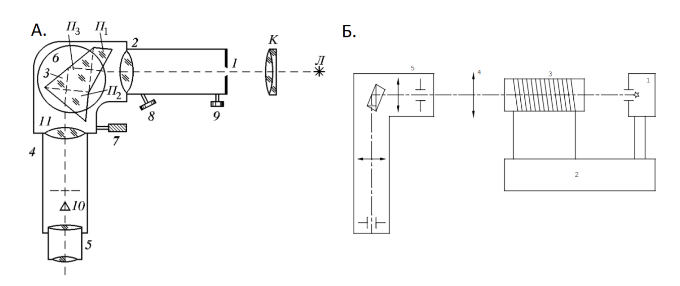
\includegraphics[width=0.5\linewidth]{p1.png}
	\caption{Установки для наблюдения линий А. водорода; Б. йода}
	\label{pic_2}
\end{figure}

На Рис. 2Б изображена схема установки, используемой для наблюдения спектра йода. Спектр поглощения паров йода наблюдается визуально на фоне сплошного спектра лампы накаливания 1, питаемой от блока питания 2. Кювета 3 с кристаллами йода подогревается нихромовой спиралью, подключённой вместе с лампой накаливания к блоку питания. Линза 4 используется как конденсор. В результате подогрева кристаллы йода частично возгоняются, образуя пары
с лёгкой фиолетовой окраской. Спектрометр 5 позволяет визуально наблюдать линии поглощения молекул йода на фоне сплошного спектра излучения лампы накаливания видимой области.

\section{Ход работы}

$\textbf{1.}$ Построил грудуировочную кривую слудующим образом: по оси X отложил градусные деления барабана, а по оси Y длины волн соответствующих линий. 

\begin{figure}[!hb]
	\centering
	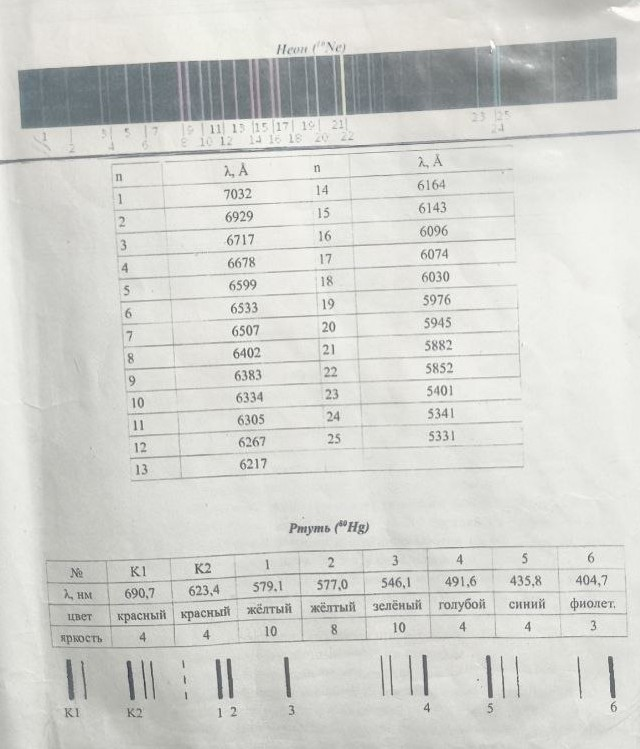
\includegraphics[width=0.4\linewidth]{p5.jpg}
	\caption{Таблица для опереления длин волн}
	\label{pic_2}
\end{figure}

\newpage

% \begin{figure}[!hb]
% 	\centering
% 	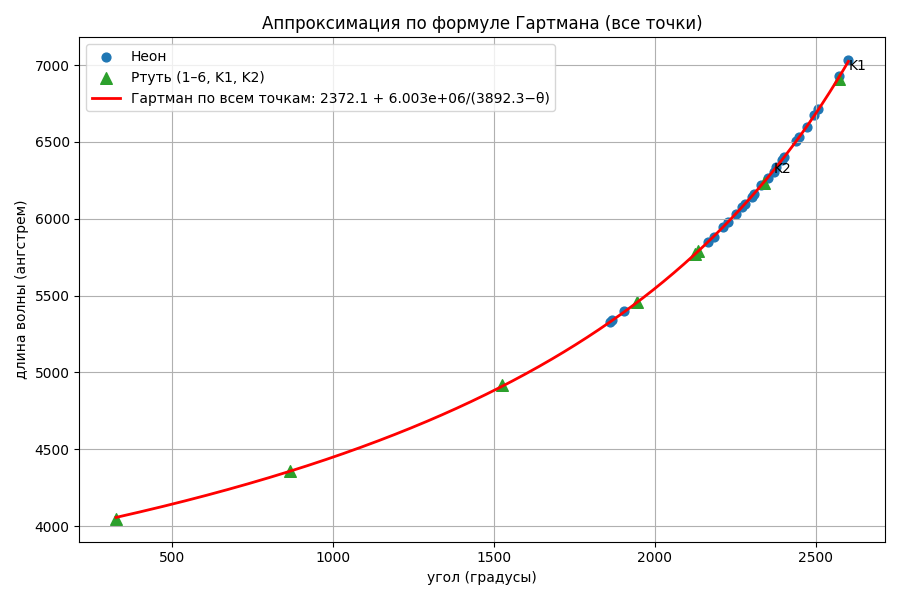
\includegraphics[width=0.4\linewidth]{F1.png}
% 	\caption{График зависимости $\lambda (\theta)$}
% 	\label{pic_2}
% \end{figure}


\begin{landscape}
  \begin{figure}[p]              % [p] — вынести на отдельную страницу
    \centering
    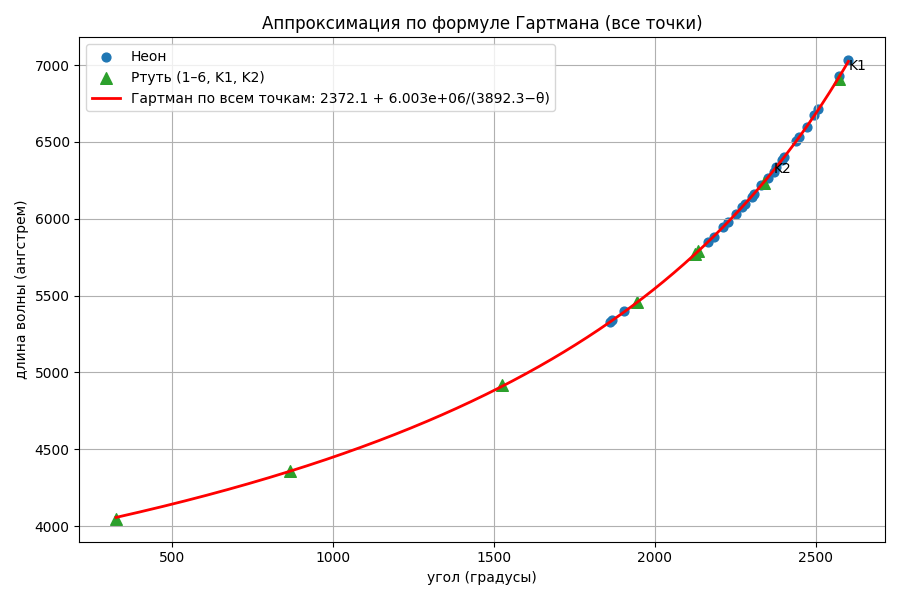
\includegraphics[width=\linewidth,height=0.9\textheight,keepaspectratio]{F1.png}
    \caption{График зависимости $\lambda (\theta)$}
    \label{fig:wide}
  \end{figure}
\end{landscape}

\newpage

$\textbf{2.}$ Из графика определим длину волны для $H_{\alpha}, H_{\beta}, H_{\gamma}, H_{\delta} $:

\begin{itemize}
	\item $H_{\alpha}$: 6566 ангстремм (2460 градусов)
	\item $H_{\beta}$: 4857 ангмтремм (1476 градусов)
	\item $H_{\gamma}$: 4337 ангстремм (837 градусов)
	\item $H_{\delta}$: 4100 ангстремм (417 грудусов)
\end{itemize}

$\textbf{3.}$ Проверка сериальной закономерности: \par

Для атома водорода серия Бальмера описывается формулой:
\[
\frac{1}{\lambda} = R \left( \frac{1}{2^2} - \frac{1}{n^2} \right), \quad n = 3, 4, 5, 6, \ldots
\]

Постоянная Ридберга $R$ одинакова для всех линий. Поэтому отношения длин волн не должны зависеть от $R$. Из формулы:
\[
\lambda = \frac{1}{R \left( \frac{1}{4} - \frac{1}{n^2} \right)}
\]
Тогда отношение двух длин волн:
\[
\frac{\lambda_i}{\lambda_j} = \frac{\frac{1}{4} - \frac{1}{n_j^2}}{\frac{1}{4} - \frac{1}{n_i^2}}
\]

Построим график $\frac{1}{\lambda} (\frac{1}{4} - \frac{1}{n^{2}})$ и убедимся, что точки ложатся на прямую линию:

\begin{figure}[!hb]
	\centering
	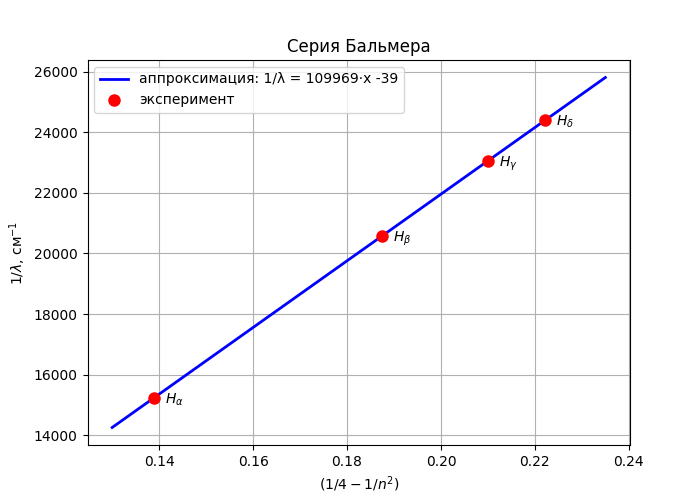
\includegraphics[width=0.7\linewidth]{F2.png}
	\caption{$\frac{1}{\lambda} (\frac{1}{4} - \frac{1}{n^{2}})$}
	\label{pic_2}
\end{figure}

Из наклона прямой можно найти постоянную Ридберга : $R_{y} = 109969$ $\text{см}^{-1}$ при табличном значении $R_{y} = 109737$ $\text{см}^{-1}$

$\textbf{4.}$ Вычисление постоянной Ридберга \par

По формуле посчитаем для каждой линии водорода постоянную Ридберга:

\[
R = \frac{1}{\lambda \left( \frac{1}{4} - \frac{1}{n^2} \right)}
\]


\subsection*{Линия $H_\alpha$ ($n=3$, $\lambda = 6566$ \AA)}
\begin{align}
R &= \frac{1}{6566 \times 10^{-10} \left(\frac{1}{4} - \frac{1}{9}\right)} \\
&= \frac{1}{6566 \times 10^{-10} \cdot \frac{5}{36}} \\
&= \frac{36}{6566 \times 10^{-10} \cdot 5} \\
&= \frac{36}{3.283 \times 10^{-6}} \\
&\approx 1.097 \times 10^7 \text{ м}^{-1}
\end{align}

\subsection*{Линия $H_\beta$ ($n=4$, $\lambda = 4857$ \AA)}
\begin{align}
R &= \frac{1}{4857 \times 10^{-10} \left(\frac{1}{4} - \frac{1}{16}\right)} \\
&= \frac{1}{4857 \times 10^{-10} \cdot \frac{3}{16}} \\
&= \frac{16}{4857 \times 10^{-10} \cdot 3} \\
&= \frac{16}{1.457 \times 10^{-6}} \\
&\approx 1.098 \times 10^7 \text{ м}^{-1}
\end{align}

\subsection*{Линия $H_\gamma$ ($n=5$, $\lambda = 4337$ \AA)}
\begin{align}
R &= \frac{1}{4337 \times 10^{-10} \left(\frac{1}{4} - \frac{1}{25}\right)} \\
&= \frac{1}{4337 \times 10^{-10} \cdot \frac{21}{100}} \\
&= \frac{100}{4337 \times 10^{-10} \cdot 21} \\
&= \frac{100}{9.108 \times 10^{-7}} \\
&\approx 1.098 \times 10^7 \text{ м}^{-1}
\end{align}

\subsection*{Линия $H_\delta$ ($n=6$, $\lambda = 4100$ \AA)}
\begin{align}
R &= \frac{1}{4100 \times 10^{-10} \left(\frac{1}{4} - \frac{1}{36}\right)} \\
&= \frac{1}{4100 \times 10^{-10} \cdot \frac{8}{36}} \\
&= \frac{36}{4100 \times 10^{-10} \cdot 8} \\
&= \frac{36}{3.280 \times 10^{-6}} \\
&\approx 1.098 \times 10^7 \text{ м}^{-1}
\end{align}

По формуле Найдем среднее значение:

\begin{equation}
\bar{R} = \frac{R_\alpha + R_\beta + R_\gamma + R_\delta}{4}
\end{equation}

Подстановка значений:
\begin{align}
\bar{R} &= \frac{1.097 \times 10^7 + 1.098 \times 10^7 + 1.098 \times 10^7 + 1.098 \times 10^7}{4} \text{ м}^{-1} \\[10pt]
&= \frac{(1.097 + 1.098 + 1.098 + 1.098) \times 10^7}{4} \text{ м}^{-1} \\[10pt]
&= \frac{4.391 \times 10^7}{4} \text{ м}^{-1} \\[10pt]
&\approx 1.098 \times 10^7 \text{ м}^{-1}
\end{align}

\textbf{Результат:} $\bar{R} \approx 1.098 \times 10^7$ м$^{-1}$

Табличное значение: $R = 1.097 \times 10^7$ м$^{-1}$

Относительная погрешность:
\begin{equation}
\varepsilon = \frac{|\bar{R} - R_{\text{табл}}|}{R_{\text{табл}}} \times 100\% = \frac{|1.098 - 1.097| \times 10^7}{1.097 \times 10^7} \times 100\% \approx 0.09\%
\end{equation}

Определим погрешность:

$N = 4$, $\bar{R} = 1.09775 \times 10^7$ м$^{-1}$

$\textbf{Стандартное отклонение}$
\begin{align}
s &= \sqrt{\frac{\sum(R_i - \bar{R})^2}{N - 1}} \\
&= \sqrt{\frac{(1.097-1.09775)^2 + (1.098-1.09775)^2 + (1.098-1.09775)^2 + (1.098-1.09775)^2}{3}} \times 10^7 \\
&= \sqrt{\frac{(-0.00075)^2 + (0.00025)^2 + (0.00025)^2 + (0.00025)^2}{3}} \times 10^7 \\
&= \sqrt{\frac{7.5 \times 10^{-7}}{3}} \times 10^7 \\
&= \sqrt{2.5 \times 10^{-7}} \times 10^7 \\
&= 5 \times 10^3 \text{ м}^{-1}
\end{align}

$\textbf{Стандартная оштбка среднего}$
\begin{align}
\sigma_{\bar{R}} &= \frac{s}{\sqrt{N}} = \frac{5 \times 10^3}{\sqrt{4}} = \frac{5 \times 10^3}{2} = 2.5 \times 10^3 \text{ м}^{-1}
\end{align}

$\textbf{Итог}$
\begin{equation}
\bar{R} = (1.098 \pm 0.003) \times 10^7 \text{ м}^{-1}
\end{equation}

$\textbf{5.}$ Определение длин волн линий поглощения йода \par

\begin{itemize}
	\item $n_{1,0} = 2224$ $\lambda_{1,0} = 5971$
	\item $n_{1,5} = 2118$ $\lambda_{1,5} = 5756$
	\item $n_{\text{гр}} = 1736$ $\lambda_{\text{гр}} = 5157$
\end{itemize}

$\textbf{6.}$  Энергия колебательного кванта возбуждённого состояния

\[
h\nu_2 = \frac{h\nu_{1,5} - h\nu_{1,0}}{5}
\]

Расчет энергии $h\nu_2$

\begin{itemize}
    \item $\lambda_{1,0} = 5971$ \AA, \quad $\lambda_{1,5} = 5756$ \AA
\end{itemize}

Вычисление $h\nu_{1,0}$ и $h\nu_{1,5}$
\begin{align}
h\nu_{1,0} &= \frac{1240}{\lambda_{1,0}} = \frac{1240}{597,1} \approx 2,077 \text{ эВ} \\[8pt]
h\nu_{1,5} &= \frac{1240}{\lambda_{1,5}} = \frac{1240}{575,6} \approx 2,154 \text{ эВ}
\end{align}

Подстановка в формулу для $h\nu_2$
\begin{align}
h\nu_2 &= \frac{h\nu_{1,5} - h\nu_{1,0}}{5} \\[8pt]
&= \frac{2,154 - 2,077}{5} \\[8pt]
&= \frac{0.077}{5} \\[8pt]
&\approx 0.0154 \text{ эВ}
\end{align}

\textbf{Результат:} $h\nu_2 \approx 15,4 \times 10^{-3}$ эВ $\approx 15$ мэВ

$\textbf{7.}$ Энергия электронного перехода и энергии диссоциации \par
а)
\[
h\nu_{\text{эл}} = h\nu_{1,0} + \frac{h\nu_1 - h\nu_2}{2}
\]

Подстановка значений:
\begin{align}
h\nu_{\text{эл}} &= 2,077 + \frac{0.027 - 0.0154}{2} \\[8pt]
&= 2,077 + 0.01273 \\[8pt]
&\approx 2,0828 \text{ эВ}
\end{align}

\textbf{Результат:} $h\nu_{\text{эл}} \approx 2,0828$ эВ

б) Энергия диссоциации в основном состоянии $D_{1}$

Баланс энергии:
\[
h\nu_{\text{тр}} = D_1 + E_A - \frac{1}{2} h\nu_1
\]

Отсюда:
\[
D_1 = h\nu_{\text{тр}} - E_A + \frac{1}{2} h\nu_1
\]

Подстановка значений:
\begin{align}
D_1 &= 2.404 - 0.94 + \frac{0.027}{2} \\[8pt]
&= 2.404 - 0.94 + 0.0135 \\[8pt]
&= 1.464 + 0.0135 \\[8pt]
&= 1.4775 \text{ эВ}
\end{align}

\textbf{Результат:} $D_1 \approx 1.48$ эВ

в) \par

\[
D_2 = D_1 + E_A - h\nu_{\text{эл}}
\]

Подстановка значений:
\begin{align}
D_2 &= 1.48 + 0.94 - 2.0828 \\[8pt]
&= 2.42 - 2.0828 \\[8pt]
&= 0.3372 \text{ эВ}
\end{align}

\textbf{Результат:} $D_2 \approx 0.34$ эВ

$\textbf{8.}$ Оценка достоверности \par

Дано, что $I_{2}$ = 1,5 эВ, что хорошо совпадает с рассчитаным $D_{1}$ \par

Известное $h\nu_{\text{гр}}$ = 2,44 совпадает с измеренным:$h\nu_{\text{гр}}$ = 2,404 эВ \par

\section{Вывод}

Измерил спектры поглощения паров йода, выделил серии электронно - колебательных переходов, определил параметры потенциала межъядерного взаимодействия в двухатомной молекуле йода.



\end{document}